\chapter{Convolutional Neural Networks}
\label{chap:convolutional_networks}

\section*{Chapter Overview}

Convolutional Neural Networks (CNNs) revolutionized computer vision by exploiting spatial structure. This chapter develops convolution operations, pooling, and modern CNN architectures including ResNet.

\subsection*{Learning Objectives}

\begin{enumerate}
    \item Understand convolution operations and compute output dimensions
    \item Design CNN architectures with appropriate pooling and stride
    \item Understand translation equivariance
    \item Implement modern CNN architectures (ResNet, VGG)
\end{enumerate}

\section{Convolution Operation}
\label{sec:convolution_operation}

\begin{definition}[2D Convolution]
\label{def:2d_convolution}
For input $\mX \in \R^{H \times W}$ and kernel $\mK \in \R^{k_h \times k_w}$:
\begin{equation}
(\mX \star \mK)_{i,j} = \sum_{m=0}^{k_h-1} \sum_{n=0}^{k_w-1} \mX_{i+m, j+n} \cdot \mK_{m,n}

\begin{mermaid}[CNN Forward Pass with Memory]
graph LR
    X["Input\n X in R^H x W x C_in"] -->|"Filters K in R^k x k x C_in x C_out\n bias b in R^C_out"| CONV["Conv2D\n (X * K + b)\n Output in R^H' x W' x C_out\n STORED: X for dL/dK"]
    CONV -->|"ReLU"| ACT["Activation\n ReLU(conv)\n in R^H' x W' x C_out\n STORED: conv for ReLU'"]
    ACT -->|"stride s, pool size p"| POOL["MaxPool\n in R^H'' x W'' x C_out\n STORED: max indices\n for backprop routing"]
    POOL -->|"Flatten"| FLAT["Flat vector\n in R^(H''*W''*C_out)"]
    FLAT -->|"W_fc in R^K x D\n b_fc in R^K"| FC["FC Layer\n z = W_fc * flat + b_fc\n in R^K\n STORED: flat for dL/dW"]
    FC -->|"softmax"| OUT["Output\n y_hat in R^K"]

    style X fill:#e8f5e9,stroke:#4caf50,color:#000
    style CONV fill:#fff3e0,stroke:#ff9800,color:#000
    style ACT fill:#e3f2fd,stroke:#2196f3,color:#000
    style POOL fill:#fff3e0,stroke:#ff9800,color:#000
    style FC fill:#e3f2fd,stroke:#2196f3,color:#000
    style OUT fill:#f3e5f5,stroke:#9c27b0,color:#000
\end{mermaid}

\end{equation}
\end{definition}

\begin{figure}[h]
\centering
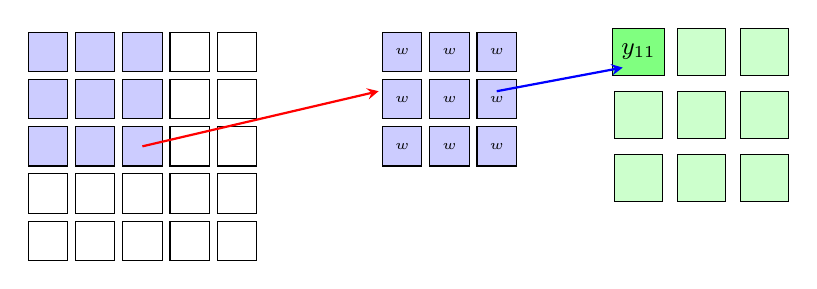
\begin{tikzpicture}[
    cell/.style={rectangle, draw, minimum size=0.5cm, font=\tiny},
    kernel/.style={rectangle, draw, fill=blue!20, minimum size=0.5cm, font=\tiny},
    output/.style={rectangle, draw, fill=green!20, minimum size=0.6cm, font=\small},
    arrow/.style={->, >=stealth, thick}
]

% Input feature map (5x5)
\foreach \i in {0,...,4} {
    \foreach \j in {0,...,4} {
        \node[cell] (in\i\j) at (\j*0.6, -\i*0.6) {};
    }
}

% Highlight receptive field for first output
\foreach \i in {0,1,2} {
    \foreach \j in {0,1,2} {
        \node[kernel] at (\j*0.6, -\i*0.6) {};
    }
}

% 3x3 Kernel
\foreach \i in {0,1,2} {
    \foreach \j in {0,1,2} {
        \node[kernel] (k\i\j) at (4.5+\j*0.6, -\i*0.6) {$w$};
    }
}

% Output feature map (3x3)
\foreach \i in {0,1,2} {
    \foreach \j in {0,1,2} {
        \node[output] (out\i\j) at (7.5+\j*0.8, -\i*0.8) {};
    }
}

% Highlight first output
\node[output, fill=green!50] at (7.5, 0) {$y_{11}$};

% Arrows showing receptive field
\draw[arrow, red, thick] (1.2, -1.2) -- (4.2, -0.5);
\draw[arrow, blue, thick] (5.7, -0.5) -- (7.3, -0.2);

\end{tikzpicture}
\caption{CNN receptive field showing local connectivity. Each output neuron connects to a local $3 \times 3$ region of the input (highlighted in blue), not all inputs. The same kernel weights are shared across all spatial positions, enabling parameter efficiency and translation invariance.}

\textbf{Convolution:} Only $3 \times 3 = 9$ connections (parameter sharing!)

\caption{Convolutional layer receptive field showing local connectivity. Each output neuron (green) connects only to a local $3 \times 3$ patch of the input (blue highlighted region), not to all input positions. The same $3 \times 3$ kernel weights are shared across all spatial positions, dramatically reducing parameters compared to fully-connected layers. For a $5 \times 5$ input, a fully-connected layer would require 25 weights per output, while convolution requires only 9 weights total (shared across all outputs).}
\label{fig:conv_receptive_field}
\end{figure}

\begin{example}[3x3 Convolution]
\label{ex:3x3_conv}
Input $4\times4$, kernel $3\times3$ (edge detector), output $2\times2$. Computing first position: sum of element-wise products gives edge response.
\end{example}

\subsection{Output Dimensions}

\begin{theorem}[Output Size]
\label{thm:conv_output_size}
For input size $H \times W$, kernel $k_h \times k_w$, padding $p$, stride $s$:
\begin{equation}
H_{\text{out}} = \left\lfloor \frac{H + 2p - k_h}{s} \right\rfloor + 1
\end{equation}
\end{theorem}

\section{Multi-Channel Convolutions}
\label{sec:multi_channel}

\begin{definition}[Convolutional Layer]
\label{def:conv_layer}
For input $\mathbf{X} \in \R^{C_{\text{in}} \times H \times W}$ with $C_{\text{out}}$ output channels:
\begin{equation}
\mathbf{Y}^{(i)} = \sum_{c=1}^{C_{\text{in}}} \mathbf{X}^{(c)} \star \mathbf{K}^{(i,c)} + b^{(i)}
\end{equation}
\end{definition}

\begin{example}[RGB Convolution]
\label{ex:rgb_conv}
Input: $\mathbf{X} \in \R^{3 \times 224 \times 224}$. Conv layer: 64 filters $3\times3$, stride 1, padding 1.

Parameters: $64 \times 3 \times 3 \times 3 + 64 = 1{,}792$

Output: $\mathbf{Y} \in \R^{64 \times 224 \times 224}$

Compare to fully-connected: $\approx 483$ billion parameters!
\end{example}

\begin{keypoint}
Convolution provides: (1) Parameter sharing, (2) Local connectivity, (3) Translation equivariance. Massive parameter reduction compared to fully-connected layers.
\end{keypoint}

\section{Computational Analysis of Convolutions}
\label{sec:conv_computation}

Understanding the computational cost and memory requirements of convolutional layers is essential for designing efficient architectures and comparing CNNs with alternative approaches like transformers. The relationship between parameters, FLOPs, and memory usage in convolutions differs fundamentally from fully-connected layers, leading to distinct performance characteristics on modern hardware.

\subsection{FLOPs for Convolution Operations}

The computational cost of a convolutional layer is determined by the number of multiply-accumulate operations required to compute all output feature maps. For a convolutional layer with input shape $C_{\text{in}} \times H \times W$, kernel size $k \times k$, and $C_{\text{out}}$ output channels, each output position requires $C_{\text{in}} \times k \times k$ multiply-accumulate operations. With output spatial dimensions $H_{\text{out}} \times W_{\text{out}}$ and $C_{\text{out}}$ output channels, the total FLOPs is:

\begin{equation}
\text{FLOPs}_{\text{conv}} = 2 \times C_{\text{out}} \times C_{\text{in}} \times k^2 \times H_{\text{out}} \times W_{\text{out}}
\end{equation}

The factor of 2 accounts for the multiply-accumulate operation (one multiplication and one addition per operation). This formula reveals that convolution FLOPs scale linearly with both input and output channels, quadratically with kernel size, and linearly with output spatial dimensions.

For the RGB convolution example in Example~\ref{ex:rgb_conv} with input $3 \times 224 \times 224$, kernel size $3 \times 3$, and 64 output channels with stride 1 and padding 1, the output dimensions are $64 \times 224 \times 224$. The FLOPs calculation is $2 \times 64 \times 3 \times 9 \times 224 \times 224 = 173{,}408{,}192$ FLOPs, or approximately 173 MFLOPs. Despite having only 1,792 parameters, this layer requires 173 million floating-point operations, giving a FLOPs-to-parameter ratio of approximately 96,768. This ratio is dramatically higher than fully-connected layers, which have a FLOPs-to-parameter ratio of approximately 2-3.

The high FLOPs-to-parameter ratio of convolutions has important implications for model design. Convolutional layers are compute-intensive relative to their memory footprint, making them well-suited for modern GPUs that have abundant compute throughput but limited memory bandwidth. A ResNet-50 model with 25.6 million parameters requires approximately 4.1 billion FLOPs for a single forward pass on a $224 \times 224$ image, giving an overall FLOPs-to-parameter ratio of 160. This means that during training, the computational cost dominates over the memory cost of loading parameters, and GPU utilization is primarily limited by compute throughput rather than memory bandwidth.

The scaling behavior of convolution FLOPs explains several architectural design choices in modern CNNs. Early layers operating on high-resolution feature maps ($224 \times 224$ or larger) consume the majority of FLOPs despite having relatively few parameters. For ResNet-50, the first convolutional layer with kernel size $7 \times 7$ and 64 output channels accounts for only 0.4\% of parameters but 5.8\% of total FLOPs. Conversely, later layers operating on low-resolution feature maps ($7 \times 7$ or smaller) have many parameters but relatively few FLOPs. The final fully-connected layer in ResNet-50 accounts for 7.8\% of parameters but only 0.1\% of FLOPs. This distribution motivates the use of larger kernels and more channels in early layers (where spatial dimensions are large) and smaller kernels with many channels in later layers (where spatial dimensions are small).

\subsection{Memory Requirements for Feature Maps}

During training, convolutional networks must store intermediate feature maps for use in the backward pass, and these activations typically consume far more memory than the model parameters. Understanding activation memory is critical for determining maximum batch size and input resolution.

For a convolutional layer with input shape $B \times C_{\text{in}} \times H \times W$ (where $B$ is batch size) and output shape $B \times C_{\text{out}} \times H_{\text{out}} \times W_{\text{out}}$, the network must store both the input feature map and the output feature map. In FP32, this requires $4B(C_{\text{in}} HW + C_{\text{out}} H_{\text{out}} W_{\text{out}})$ bytes of memory. For the RGB convolution example with batch size $B = 32$, input $3 \times 224 \times 224$, and output $64 \times 224 \times 224$, the activation memory is $4 \times 32 \times (3 \times 224 \times 224 + 64 \times 224 \times 224) = 130{,}809{,}792$ bytes, or approximately 125 MB. This is 70,000× larger than the parameter memory (1,792 parameters = 7,168 bytes), demonstrating that activation memory dominates for convolutional layers.

The memory consumption of a full CNN scales with the number of layers and the spatial dimensions of feature maps. For ResNet-50 processing batch size 32 with input $3 \times 224 \times 224$, the total activation memory is approximately 8.2 GB in FP32. This includes the input image (6.4 MB), early high-resolution feature maps (hundreds of MB), and later low-resolution feature maps (tens of MB). The parameter memory for ResNet-50 is only 102 MB (25.6 million parameters × 4 bytes), making activations 80× larger than parameters. This ratio increases with batch size: at batch size 256, activations consume 65.6 GB while parameters remain 102 MB, a ratio of 643×.

The quadratic scaling of activation memory with spatial resolution has profound implications for input image size. Doubling the input resolution from $224 \times 224$ to $448 \times 448$ increases the number of pixels by 4×, and since early feature maps maintain similar spatial dimensions to the input, activation memory increases by approximately 4×. For ResNet-50 with batch size 32, increasing resolution from $224 \times 224$ to $448 \times 448$ increases activation memory from 8.2 GB to approximately 32.8 GB, exceeding the capacity of most GPUs. This explains why high-resolution image processing typically requires smaller batch sizes or gradient accumulation: the activation memory grows faster than available GPU memory.

Modern techniques for reducing activation memory include gradient checkpointing, which recomputes activations during the backward pass rather than storing them, trading computation for memory. For ResNet-50, gradient checkpointing can reduce activation memory by 5-10× at the cost of increasing training time by 20-30\%. This trade-off is often worthwhile for training with larger batch sizes or higher resolutions, as the improved convergence from larger batches can offset the increased computation time.

\subsection{GPU Optimization: im2col and Winograd}

Efficient implementation of convolution on GPUs requires specialized algorithms that transform the convolution operation into a form amenable to highly optimized matrix multiplication routines. The two primary approaches are im2col (image-to-column) and Winograd convolution, each with distinct performance characteristics.

The im2col algorithm transforms convolution into matrix multiplication by unrolling the input feature map into a large matrix where each column contains the input values for one output position. For a convolutional layer with input $C_{\text{in}} \times H \times W$, kernel size $k \times k$, and output $C_{\text{out}} \times H_{\text{out}} \times W_{\text{out}}$, im2col creates a matrix of shape $(C_{\text{in}} k^2) \times (H_{\text{out}} W_{\text{out}})$ by extracting all $k \times k$ patches from the input. The convolution kernels are reshaped into a matrix of shape $C_{\text{out}} \times (C_{\text{in}} k^2)$. The convolution is then computed as a single matrix multiplication: $\text{output} = \text{kernels} \times \text{im2col}(\text{input})$, producing a matrix of shape $C_{\text{out}} \times (H_{\text{out}} W_{\text{out}})$ that is reshaped to the final output dimensions.

For the RGB convolution example with input $3 \times 224 \times 224$, kernel size $3 \times 3$, and 64 output channels, im2col creates a matrix of shape $27 \times 50{,}176$ (since $C_{\text{in}} k^2 = 3 \times 9 = 27$ and $H_{\text{out}} W_{\text{out}} = 224 \times 224 = 50{,}176$). The kernel matrix has shape $64 \times 27$. The matrix multiplication $64 \times 27$ times $27 \times 50{,}176$ requires $2 \times 64 \times 27 \times 50{,}176 = 173{,}408{,}192$ FLOPs, matching the direct convolution calculation. However, the im2col matrix requires $27 \times 50{,}176 \times 4 = 5{,}419{,}008$ bytes (5.2 MB) of temporary storage, which is 757× larger than the original input (7,168 bytes for $3 \times 224 \times 224$ in FP32).

The advantage of im2col is that it leverages highly optimized BLAS (Basic Linear Algebra Subprograms) libraries like cuBLAS on NVIDIA GPUs, which achieve 80-95\% of peak hardware throughput for large matrix multiplications. For the $64 \times 27$ times $27 \times 50{,}176$ multiplication on an NVIDIA A100 GPU with 312 TFLOPS FP16 throughput, the operation completes in approximately 0.6 microseconds at 90\% efficiency, achieving 280 TFLOPS. Direct convolution implementations without im2col typically achieve only 40-60\% efficiency due to irregular memory access patterns and difficulty saturating the GPU's parallel execution units.

The disadvantage of im2col is the memory overhead. For batch size $B = 32$, the im2col matrix grows to $32 \times 27 \times 50{,}176 = 43{,}352{,}064$ elements, requiring 167 MB of temporary storage. This memory must be allocated and deallocated for each convolutional layer, adding memory pressure and potentially causing out-of-memory errors for large batch sizes or high-resolution inputs. Modern implementations mitigate this by processing the batch in chunks or fusing the im2col transformation with the matrix multiplication to avoid materializing the full im2col matrix.

Winograd convolution is an alternative algorithm that reduces the number of multiplications required for small convolutions (typically $3 \times 3$ or $5 \times 5$ kernels) by using a mathematical transformation that trades multiplications for additions. For $3 \times 3$ convolutions, Winograd reduces the number of multiplications by 2.25× compared to direct convolution, from 9 multiplications per output to 4 multiplications per output. This reduction translates directly to FLOPs savings: the RGB convolution example requires only $173{,}408{,}192 / 2.25 = 77{,}070{,}752$ FLOPs with Winograd, a 56\% reduction.

However, Winograd convolution has several limitations. First, it requires additional memory for intermediate transformations, typically 2-3× the input size. Second, it is numerically less stable than direct convolution, particularly in FP16, due to the transformation matrices having large condition numbers. Third, it is only applicable to small kernel sizes ($3 \times 3$ and $5 \times 5$) and becomes inefficient for larger kernels. Fourth, the transformation overhead becomes significant for small spatial dimensions, making Winograd most effective for early layers with large feature maps.

In practice, modern deep learning frameworks like PyTorch and TensorFlow automatically select between im2col, Winograd, and direct convolution based on layer dimensions, batch size, and hardware characteristics. For $3 \times 3$ convolutions on high-resolution feature maps ($\geq 56 \times 56$) with batch size $\geq 16$, Winograd typically provides 1.5-2× speedup over im2col. For larger kernels ($5 \times 5$ or $7 \times 7$) or smaller feature maps, im2col is preferred. For very small batch sizes ($\leq 4$), direct convolution may be fastest due to lower overhead. NVIDIA's cuDNN library implements all three algorithms and includes heuristics to select the optimal approach for each layer configuration.

\subsection{Comparison with Transformer Attention}

Comparing the computational characteristics of convolutional layers with transformer self-attention reveals fundamental trade-offs between local and global receptive fields, parameter efficiency, and computational scaling.

A convolutional layer with kernel size $k \times k$ has a local receptive field: each output position depends only on a $k \times k$ neighborhood of the input. To achieve a global receptive field spanning the entire input, multiple convolutional layers must be stacked. For an input of size $H \times W$, achieving a receptive field covering the full input requires approximately $\log_k(\max(H, W))$ layers. For a $224 \times 224$ image with $3 \times 3$ convolutions, this requires approximately $\log_3(224) \approx 5$ layers. Each layer adds computational cost, but the cost per layer remains $O(C_{\text{out}} C_{\text{in}} k^2 HW)$, scaling linearly with spatial dimensions.

In contrast, self-attention in transformers has a global receptive field: each output position attends to all input positions in a single layer. For an input sequence of length $n = HW$ (treating the 2D image as a 1D sequence) with model dimension $d$, self-attention requires computing query-key products for all pairs of positions, resulting in $O(n^2 d)$ FLOPs. For a $224 \times 224$ image with $n = 50{,}176$ positions and $d = 768$ (typical for Vision Transformers), self-attention requires approximately $2 \times 50{,}176^2 \times 768 = 3.86 \times 10^{12}$ FLOPs, or 3.86 TFLOPs per layer. This is 22,000× more expensive than the RGB convolution example (173 MFLOPs), despite both operating on the same input resolution.

The quadratic scaling of attention with spatial resolution makes it prohibitively expensive for high-resolution images. Doubling the resolution from $224 \times 224$ to $448 \times 448$ increases attention FLOPs by 16× (since $n$ increases by 4× and attention scales as $n^2$), while convolution FLOPs increase by only 4× (linear scaling with spatial dimensions). For a $448 \times 448$ image, self-attention requires 61.8 TFLOPs per layer, making it impractical without modifications like hierarchical attention or local attention windows.

Vision Transformers (ViTs) address this computational challenge by dividing the image into patches and treating each patch as a token. For a $224 \times 224$ image with patch size $16 \times 16$, the sequence length is $n = (224/16)^2 = 196$ patches. Self-attention on 196 patches with $d = 768$ requires $2 \times 196^2 \times 768 = 59{,}015{,}168$ FLOPs, or approximately 59 MFLOPs per layer. This is 65× less expensive than attention on individual pixels and comparable to the RGB convolution example (173 MFLOPs). However, the patch-based approach sacrifices fine-grained spatial resolution: each patch is treated as a single token, and the model cannot attend to individual pixels within a patch.

The parameter efficiency of convolutions versus attention also differs significantly. A convolutional layer with $C_{\text{in}}$ input channels, $C_{\text{out}}$ output channels, and kernel size $k \times k$ has $C_{\text{out}} C_{\text{in}} k^2$ parameters. For the RGB convolution example, this is $64 \times 3 \times 9 = 1{,}728$ parameters. A self-attention layer with model dimension $d$ has query, key, and value projection matrices, each of size $d \times d$, totaling $3d^2$ parameters (ignoring the output projection). For $d = 768$, this is $3 \times 768^2 = 1{,}769{,}472$ parameters, which is 1,024× more than the convolutional layer. However, the attention parameters are independent of spatial resolution, while convolution parameters are independent of spatial resolution as well. The key difference is that attention parameters scale with $d^2$ while convolution parameters scale with $C_{\text{in}} C_{\text{out}} k^2$, and typically $d \gg C_{\text{in}}$ for early layers.

For complete models, ResNet-50 has 25.6 million parameters and requires 4.1 GFLOPs per image, while ViT-Base has 86 million parameters and requires 17.6 GFLOPs per image. The ViT has 3.4× more parameters and 4.3× more FLOPs, but achieves comparable or better accuracy on ImageNet classification. The higher computational cost of ViT is offset by its ability to leverage large-scale pretraining on datasets like ImageNet-21k or JFT-300M, where the global receptive field and flexibility of attention provide advantages over the inductive biases of convolution.

\begin{keypoint}
CNNs are significantly more parameter-efficient than transformers for vision tasks due to weight sharing and local connectivity. ResNet-50 achieves 76.1\% ImageNet accuracy with 25.6M parameters, while ViT-Base requires 86M parameters for comparable accuracy. However, Vision Transformers excel when large-scale pretraining data is available. A detailed comparison of CNNs and Vision Transformers is provided in Chapter~17.
\end{keypoint}

\begin{keypoint}
Efficient convolution on GPUs requires channel dimensions that are multiples of 16 (for Tensor Core alignment) and sufficient batch size to saturate parallel compute units. Libraries like cuDNN automatically select optimal algorithms (im2col, Winograd, FFT) and apply kernel fusions. Early CNN layers are typically memory-bandwidth-bound while later layers are compute-bound. For a detailed treatment of hardware optimization, see Chapter~22.
\end{keypoint}

\section{Pooling Layers}
\label{sec:pooling}

\begin{definition}[Max Pooling]
\label{def:max_pooling}
For window $k \times k$ and stride $s$:
\begin{equation}
\text{MaxPool}(\mathbf{X})_{i,j} = \max_{m,n \in \text{window}} \mathbf{X}_{si+m, sj+n}
\end{equation}
\end{definition}

Pooling reduces spatial dimensions, increases receptive field, and provides translation invariance.

\section{Classic Architectures}
\label{sec:classic_architectures}

\subsection{VGG-16 (2014)}

Deep network with small $3\times3$ filters. Pattern: $[\text{Conv}3\times3]^n \to \text{MaxPool} \to \text{Double channels}$

Total: 138 million parameters

\subsection{ResNet (2015)}

\begin{definition}[Residual Block]
\label{def:residual_block}
Learn residual:
\begin{equation}
\mathbf{y} = \mathcal{F}(\mathbf{x}) + \mathbf{x}
\end{equation}
\end{definition}

ResNet-50: 25.6M parameters, enables training 100+ layer networks.

\begin{keypoint}
Residual connections enable extremely deep networks by allowing gradients to flow through skip connections. Analogous to skip connections in transformers.
\end{keypoint}

\section{Batch Normalization}
\label{sec:batch_norm}

\begin{definition}[Batch Normalization]
\label{def:batch_norm}
For mini-batch, normalize each feature:
\begin{align}
\hat{\mathbf{x}}_i &= \frac{\mathbf{x}_i - \mu_{\mathcal{B}}}{\sqrt{\sigma^2_{\mathcal{B}} + \epsilon}} \\
\mathbf{y}_i &= \gamma \hat{\mathbf{x}}_i + \beta
\end{align}
where $\gamma, \beta$ are learnable.
\end{definition}

Benefits: Reduces covariate shift, allows higher learning rates, acts as regularization.

\section{Exercises}

\begin{exercise}
For $32\times32\times3$ input, compute dimensions after: Conv(64, $5\times5$, s=1, p=2), MaxPool($2\times2$, s=2), Conv(128, $3\times3$, s=1, p=1), MaxPool($2\times2$, s=2). Count parameters.
\end{exercise}

\begin{exercise}
Show two $3\times3$ convolutions equal one $5\times5$ receptive field. Compare parameter counts.
\end{exercise}

\begin{exercise}
Design CNN for CIFAR-10 with 3 blocks, channels [64, 128, 256]. Calculate total parameters.
\end{exercise}

\section{Solutions}

Full solutions for all exercises are available at \url{https://deeplearning.hofkensvermeulen.be}.

\begin{solution}[Exercise 1]
Starting with input $32\times32\times3$:

\textbf{Conv1 (64 filters, $5\times5$, stride=1, padding=2):}
\begin{equation}
H_{\text{out}} = \frac{32 + 2(2) - 5}{1} + 1 = \frac{32 + 4 - 5}{1} + 1 = 32
\end{equation}
Output: $32\times32\times64$

Parameters: $(5 \times 5 \times 3 + 1) \times 64 = 76 \times 64 = 4{,}864$

\textbf{MaxPool1 ($2\times2$, stride=2):}
\begin{equation}
H_{\text{out}} = \frac{32 - 2}{2} + 1 = 16
\end{equation}
Output: $16\times16\times64$

Parameters: 0 (pooling has no learnable parameters)

\textbf{Conv2 (128 filters, $3\times3$, stride=1, padding=1):}
\begin{equation}
H_{\text{out}} = \frac{16 + 2(1) - 3}{1} + 1 = 16
\end{equation}
Output: $16\times16\times128$

Parameters: $(3 \times 3 \times 64 + 1) \times 128 = 577 \times 128 = 73{,}856$

\textbf{MaxPool2 ($2\times2$, stride=2):}
\begin{equation}
H_{\text{out}} = \frac{16 - 2}{2} + 1 = 8
\end{equation}
Output: $8\times8\times128$

\textbf{Total parameters:} $4{,}864 + 73{,}856 = 78{,}720$
\end{solution}

\begin{solution}[Exercise 2]
\textbf{Receptive field analysis:}

\textbf{Single $5\times5$ convolution:}
\begin{itemize}
    \item Receptive field: $5\times5 = 25$ pixels
    \item Parameters per output channel: $5 \times 5 \times C_{\text{in}} + 1$
    \item For $C_{\text{in}} = C_{\text{out}} = 64$: $(25 \times 64 + 1) \times 64 = 102{,}464$ parameters
\end{itemize}

\textbf{Two $3\times3$ convolutions:}
\begin{itemize}
    \item First $3\times3$ conv: receptive field $3\times3$
    \item Second $3\times3$ conv: each output pixel sees $3\times3$ region of previous layer
    \item Each pixel in previous layer sees $3\times3$ region of input
    \item Total receptive field: $3 + (3-1) = 5$ in each dimension, so $5\times5$
\end{itemize}

\textbf{Parameter count for two $3\times3$ convolutions:}
\begin{itemize}
    \item First conv: $(3 \times 3 \times 64 + 1) \times 64 = 36{,}928$ parameters
    \item Second conv: $(3 \times 3 \times 64 + 1) \times 64 = 36{,}928$ parameters
    \item Total: $73{,}856$ parameters
\end{itemize}

\textbf{Comparison:}
\begin{equation}
\text{Reduction} = \frac{102{,}464 - 73{,}856}{102{,}464} \approx 28\%
\end{equation}

Two $3\times3$ convolutions achieve the same receptive field as one $5\times5$ with 28\% fewer parameters, plus an additional nonlinearity between them, increasing representational power.
\end{solution}

\begin{solution}[Exercise 3]
\textbf{CNN architecture for CIFAR-10 (10 classes):}

Input: $32\times32\times3$

\textbf{Block 1 (64 channels):}
\begin{itemize}
    \item Conv: $3\times3$, 64 filters, stride=1, padding=1 $\to$ $32\times32\times64$
    \item Conv: $3\times3$, 64 filters, stride=1, padding=1 $\to$ $32\times32\times64$
    \item MaxPool: $2\times2$, stride=2 $\to$ $16\times16\times64$
\end{itemize}

Parameters:
\begin{itemize}
    \item Conv1: $(3 \times 3 \times 3 + 1) \times 64 = 1{,}792$
    \item Conv2: $(3 \times 3 \times 64 + 1) \times 64 = 36{,}928$
    \item Block 1 total: $38{,}720$
\end{itemize}

\textbf{Block 2 (128 channels):}
\begin{itemize}
    \item Conv: $3\times3$, 128 filters, stride=1, padding=1 $\to$ $16\times16\times128$
    \item Conv: $3\times3$, 128 filters, stride=1, padding=1 $\to$ $16\times16\times128$
    \item MaxPool: $2\times2$, stride=2 $\to$ $8\times8\times128$
\end{itemize}

Parameters:
\begin{itemize}
    \item Conv1: $(3 \times 3 \times 64 + 1) \times 128 = 73{,}856$
    \item Conv2: $(3 \times 3 \times 128 + 1) \times 128 = 147{,}584$
    \item Block 2 total: $221{,}440$
\end{itemize}

\textbf{Block 3 (256 channels):}
\begin{itemize}
    \item Conv: $3\times3$, 256 filters, stride=1, padding=1 $\to$ $8\times8\times256$
    \item Conv: $3\times3$, 256 filters, stride=1, padding=1 $\to$ $8\times8\times256$
    \item MaxPool: $2\times2$, stride=2 $\to$ $4\times4\times256$
\end{itemize}

Parameters:
\begin{itemize}
    \item Conv1: $(3 \times 3 \times 128 + 1) \times 256 = 295{,}168$
    \item Conv2: $(3 \times 3 \times 256 + 1) \times 256 = 590{,}080$
    \item Block 3 total: $885{,}248$
\end{itemize}

\textbf{Classifier:}
\begin{itemize}
    \item Global Average Pooling: $4\times4\times256 \to 1\times1\times256$
    \item Fully connected: $256 \to 10$
    \item Parameters: $256 \times 10 + 10 = 2{,}570$
\end{itemize}

\textbf{Total parameters:}
\begin{equation}
38{,}720 + 221{,}440 + 885{,}248 + 2{,}570 = 1{,}147{,}978 \approx 1.15\text{M parameters}
\end{equation}
\end{solution}

